\chapter{Konzept}

Das Kapitel Konzeption beschäftigt sich zunächst mit dem Prozess der Feature Extraktion. Hierfür wird der SIFT Algorithmus nach Lowe genutzt. Darauf aufbauend werden zwei Verfahren vorgestellt, das Bag of Visual Words Modell und der Autoencoder, die anhand von SIFT Deskriptoren eine Klassifizierung von Bildern ermöglichen.

\begin{enumerate}
	\item Verarbeitung der bestehenden Bilder
	\item Auswahl der Features
	\item Layer des Netzes, Stacking, Denoising ?	
\end{enumerate}

\section{Feature Extraktion}

Die Extraktion der Features ist die Basis für beide Varianten der Klassifizierung. Das Bag of Visual Words Modell nutzt die von SIFT erzeugten Feature Deskriptor für die weitere Verarbeitung. Der Autoencoder hingegen arbeitet mit Gradienten der \textit{keypoints} die vom SIFT Detektor ermittelt wurden. Aus diesem Grund werden die Feature-Vektoren und \textit{keypoints} beide berechnet und getrennt gespeichert.
Der SIFT Deskriptor enthält 128 Dimensionen und ist so für einen Vergleich nur schwer geeignet, da pro Bild ca. 100 bis 1000 Feature Vektoren generiert werden. Es werden daher im folgenden zwei Ansätze vorgestellt, die die Dimensionalität der Features reduzieren und eine durch Grafikkarten gestützte Berechnung von ähnlichen Bildern ermöglichen.

\begin{enumerate}
	\item Hier nochmal etwas auf SIFT eingehen (Funktionsweise)?
	\item Mehr zum Prozess sagen? Woher die Bilder kommen
	\item TODO: Wie werden Bilder gespeichert? Format, Platte / DB?
\end{enumerate}

\section{Ansatz 1: Bag of Visual Words}

In der Analyse wurde bereits sequentielle Varianten des Lloyd und Histogramm Algorithmus vorgestellt und aufgezeigt, an welchen Stellen eine Parallelisierung der Berechnung durch Grafikkarten erfolgen kann. Im Folgenden wird aus diesen Informationen je Algorithmus eine parallele Version für SIMD Prozessoren abgeleitet.

\subsection{Parellisierung von Llyods Algorithmus}

Der Thread in einem Block mit der ID 0 fungiert hier als Master für die anderen Threads. Die Initialisierung der Cluster mit zufälligen Vektoren aus $v$ wird ebenfalls von diesem übernommen. In Lloyds k-means Variante kann die \textit{Labeling} Phase massiv parallelisiert werden, in dem jeder Thread die Distanz eines Features zu allen Clustern misst. Auf diese Weise werden die $n$ Features auf $p$ Prozessoren aufgeteilt.

\lstset{language=C}
\begin{lstlisting}[mathescape=true]
kmeans_gpu
	if threadId == 0
		$c_{j} = rand p_{i} \in P, j = 1,...,k, c_{j} != c_{i} ALL i != j$
	synchronize threads
	until convergence
		for each $x_{i} \in P_{threadId}$
			$l_{i} = argminD(c_{j}, p_{i})$
		synchronize threads
		if threadId == 0
			for each $p_{i} \in P$
				$c_{l_{i}} = c_{l_{i}} + p_{i}$
				$m_{l_{i}} = m_{l_{i}} + 1$
			for each $c_{j} \in C$
				$c_{j} = \frac{1}{m_{j}} c_{i}$
\end{lstlisting}



\begin{itemize}
	\item jeder Thread führt nun labeling Prozess aus 
	\item Label in n dimensionalernVektor li gespeichert, dadurch keine concurrent writes
	\item Anschließend reduction durch master um Cluster zuordnung zu aktualisieren.
	\item Zentren der Cluster werden aktualisiert, solange bis Konvergenz
\end{itemize}

\subsection{Parallele Reduzierung von Histogrammen}

TODO: Allgemeines parallel reduction Prinzip in SIMD (Pseudocode?)

\section{Aufbau des Autoencoders}

In diesem Ansatz werden zur Reduzierung der Dimensionen der Feature-Vektoren wird ein Stacked Denoising Autoencoder verwendet wie er in der Arbeit von TODO \cite{aed2016} vorgeschlagen wurde. Der Autoencoder soll eine komprimierte Darstellung der Gradientenvektoren erzielen, die aus den \textit{intereset points} berechnet werden. Da dieser Vektor 3042 Werte enthält, besitzt der Autoencoder in der Eingabeschicht 3042 Neuronen. Der Encoder des vorgeschlagenen Modells besteht aus fünf Schichten, deren Neuronenanzahl sukzessive reduziert wird, bis schließlich eine Darstellung in 36 Dimensionen erreicht wird. Abbildung \ref{img:ae_model} zeigt die Schichten des Autoencoders.

\begin{figure}
	\centering
	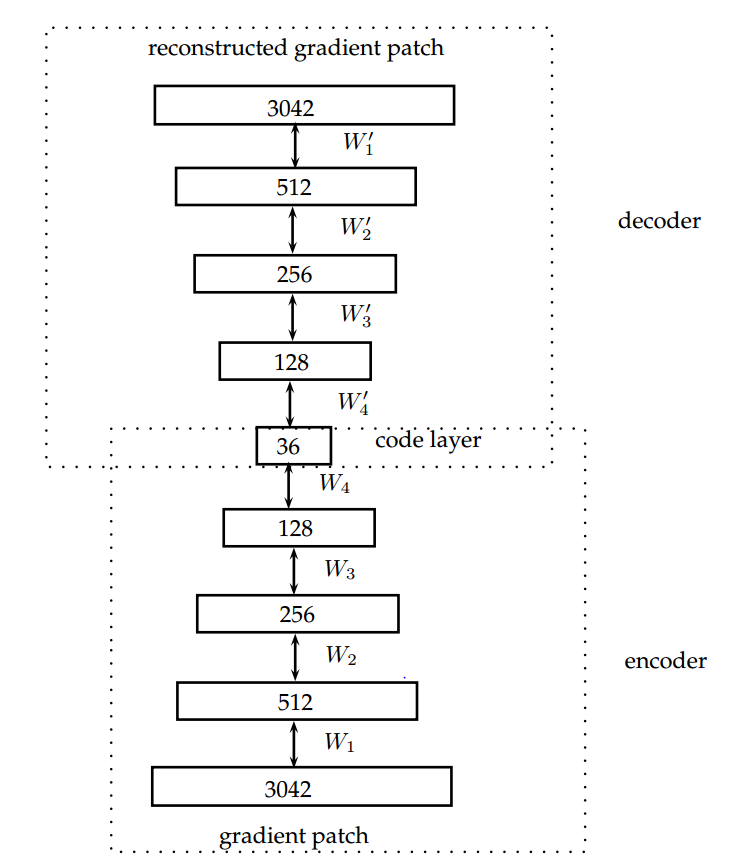
\includegraphics[scale=0.6]{images/ae_model.png}
	\caption{Schichten des verwendeten Autoencoders, Abbildung aus \cite{aed2016}}
	\label{img:ae_model}
\end{figure}

\begin{itemize}
	\item Mit Referenz auf die Arbeit ist es plausibel dieses Modell zu verwenden?
	\item In der Konzeption bereits TensorFlow erwähnen und somit Beschleunigung durch cuda Bindings?
\end{itemize}